%% ECON 282E -- Session 7, Deck A1: Machine Learning for Macroeconomists
%% Sources: AI-ECON Lec03_T1_Why_ML_Pattern_Recognition.tex, carried WHOLE
%% (13 frames); AI-ECON Lec02_T1_ML_Predictive_Stack.tex (selected);
%% Quant_Macro Lec.5 sections "Why AI/ML for Economists", "Machine Learning:
%% Overview" and "Machine Learning and Macroeconomics".
%% Figure 3.png copied into ./figures/ from Lec03_ML_for_Macro/pic/.
%% Source defects are recorded in slides/SOURCES.md, not on the slides.

%% ECON 282E -- Foundations of Macroeconomics (UC Riverside, Fall 2026)
%% Shared Beamer preamble for every deck in slides/S01 ... slides/S10.
%%
%% Usage (a deck lives in slides/S0X/ and is compiled from that folder):
%%   %% ECON 282E -- Foundations of Macroeconomics (UC Riverside, Fall 2026)
%% Shared Beamer preamble for every deck in slides/S01 ... slides/S10.
%%
%% Usage (a deck lives in slides/S0X/ and is compiled from that folder):
%%   %% ECON 282E -- Foundations of Macroeconomics (UC Riverside, Fall 2026)
%% Shared Beamer preamble for every deck in slides/S01 ... slides/S10.
%%
%% Usage (a deck lives in slides/S0X/ and is compiled from that folder):
%%   \input{../preamble/course_preamble.tex}
%%   \decktitle{1}{A1}{Who I Am \& Why This Course}{September 24, 2026}
%%   \begin{document}
%%   \makedecktitle
%%   ...
%%
%% Adapted from Courses/AI-ECON-2026/source/shared_preamble.tex (Metropolis theme,
%% concept/caution/example/takeaway boxes, \sectiondivider). Changes for this course:
%%   * course title block (\decktitle / \makedecktitle) instead of \makebeamertitle
%%   * \zh{...} typesets Chinese (book titles) under pdflatex via CJKutf8
%%   * researchbox for the "Research in the wild" frames
%%   * section pages off; TikZ libraries and the course map loaded here
%% Build with pdflatex only (two passes); tools/build_slides.py does this for you.

\documentclass[10pt,english,aspectratio=169]{beamer}

\usepackage[T1]{fontenc}
\usepackage{textcomp}
\usepackage[utf8]{inputenc}
\usepackage{babel}
\usepackage{CJKutf8}

\usepackage{amsmath, amssymb, amsthm, graphicx}
\usepackage{booktabs, multirow, tabularx}
\usepackage{tikz}
\usetikzlibrary{positioning,arrows.meta,shapes,calc,fit,backgrounds}
\usepackage{pgfplots}
\pgfplotsset{compat=1.16}
\usepackage[most]{tcolorbox}
\tcbuselibrary{skins, breakable}
\usepackage{listings}
\usepackage{xcolor}

\lstset{
  basicstyle=\ttfamily\small,
  keywordstyle=\color{blue!80!black}\bfseries,
  commentstyle=\color{green!50!black}\itshape,
  stringstyle=\color{orange!80!black},
  backgroundcolor=\color{gray!8},
  frame=single,
  rulecolor=\color{gray!40},
  breaklines=true,
  showstringspaces=false,
  numbers=none,
}

\usetheme{metropolis}
\usefonttheme{professionalfonts}
\metroset{sectionpage=none}

\definecolor{LightGray}{RGB}{230,230,230}
\definecolor{RedTitle}{RGB}{0,0,200}
\definecolor{VeryLightGray}{RGB}{245,245,245}
\definecolor{DarkText}{RGB}{0,0,0}
\definecolor{UCRBlue}{RGB}{0,45,106}
\definecolor{UCRGold}{RGB}{241,171,0}

% Stage colours of the course arc (used by the course map and elsewhere)
\colorlet{StageTrunk}{blue!12}
\colorlet{StageBranch}{cyan!14}
\colorlet{StageMachine}{gray!18}
\colorlet{StageWall}{red!14}
\colorlet{StageTools}{orange!20}
\colorlet{StageData}{green!16}
\colorlet{StageAgents}{violet!14}

\hypersetup{bookmarks=false,breaklinks=true,pdfborder={0 0 0},colorlinks=true,
  linkcolor=DarkText,urlcolor=RedTitle}

\setbeamercolor{background canvas}{bg=white}
\setbeamercolor{title}{fg=RedTitle}
\setbeamercolor{frametitle}{bg=VeryLightGray,fg=DarkText}
\setbeamercolor{normal text}{fg=DarkText}
\setbeamercolor{alerted text}{fg=RedTitle}
\setbeamersize{text margin left=5mm, text margin right=5mm}
\addtobeamertemplate{frametitle}{}{\vspace{-0.5em}}

\setbeamertemplate{navigation symbols}{}
\setbeamertemplate{footline}{%
  \hspace{5mm}{\usebeamerfont{page number in head/foot}\color{black!45}%
  ECON 282E \,$\cdot$\, \insertshortdeck}\hfill%
  \usebeamercolor[fg]{page number in head/foot}%
  \usebeamerfont{page number in head/foot}%
  \insertframenumber\,/\,\inserttotalframenumber\kern1em\vskip2pt%
}

% ---------------------------------------------------------------------------
% Chinese text under pdflatex (book titles etc.)
\newcommand{\zh}[1]{\begin{CJK*}{UTF8}{gbsn}#1\end{CJK*}}

% ---------------------------------------------------------------------------
% Deck title block
%   \decktitle{session}{deck id}{title}{date}
\newcommand{\insertshortdeck}{}
\newcommand{\decksession}{}
\newcommand{\deckid}{}
\newcommand{\decktitletext}{}
\newcommand{\deckdate}{}
\newcommand{\decktitle}[4]{%
  \renewcommand{\decksession}{#1}%
  \renewcommand{\deckid}{#2}%
  \renewcommand{\decktitletext}{#3}%
  \renewcommand{\deckdate}{#4}%
  \renewcommand{\insertshortdeck}{Session #1 \,$\cdot$\, Deck #1.#2}%
  \title{#3}%
  \author{Zhigang Feng}%
  \date{#4}%
}
\newcommand{\makedecktitle}{%
  \begin{frame}[plain,noframenumbering]
    \begin{tikzpicture}[remember picture,overlay]
      \fill[UCRBlue] (current page.north west) rectangle ([yshift=-0.55cm]current page.north east);
      \fill[UCRGold] ([yshift=-0.55cm]current page.north west) rectangle ([yshift=-0.62cm]current page.north east);
      \node[anchor=west, text=white, font=\small\bfseries] at ([xshift=5mm,yshift=-0.275cm]current page.north west)
        {ECON 282E \,$\cdot$\, Foundations of Macroeconomics};
      \node[anchor=east, text=white, font=\small] at ([xshift=-5mm,yshift=-0.275cm]current page.north east)
        {UC Riverside \,$\cdot$\, Fall 2026};
    \end{tikzpicture}
    \vspace*{1.1cm}
    {\usebeamerfont{title}\color{black!55}\large Session \decksession\ \,$\cdot$\, Deck \decksession.\deckid\par}
    \vspace{0.25cm}
    {\usebeamerfont{title}\color{RedTitle}\LARGE\bfseries \decktitletext\par}
    \vspace{0.7cm}
    {\large Zhigang Feng\par}
    \vspace{0.15cm}
    {\color{black!65}\deckdate\par}
    \vfill
    {\footnotesize\itshape\color{black!55}Build it on paper $\;\to\;$ solve it on the machine $\;\to\;$ push it to the frontier with AI\par}
  \end{frame}}

% ---------------------------------------------------------------------------
% Section divider (plain frame, not counted)
\newcommand{\sectiondivider}[2]{%
\begin{frame}[plain,noframenumbering]
\begin{center}
\vfill
{\Large\textbf{#1}\par}
\vspace{0.35cm}
{\normalsize #2\par}
\vfill
\end{center}
\end{frame}
}

% ---------------------------------------------------------------------------
% Boxes
\newtcolorbox{conceptbox}[1][]{colback=blue!3, colframe=RedTitle!55, boxrule=0.35mm,
  arc=1mm, left=2mm, right=2mm, top=1mm, bottom=1mm, #1}
\newtcolorbox{cautionbox}[1][]{colback=red!3, colframe=red!50!black, boxrule=0.35mm,
  arc=1mm, left=2mm, right=2mm, top=1mm, bottom=1mm, #1}
\newtcolorbox{examplebox}[1][]{colback=green!3, colframe=green!45!black, boxrule=0.35mm,
  arc=1mm, left=2mm, right=2mm, top=1mm, bottom=1mm, #1}
\newtcolorbox{takeawaybox}[1][]{colback=VeryLightGray, colframe=RedTitle!55, boxrule=0.35mm,
  arc=1mm, left=2mm, right=2mm, top=1mm, bottom=1mm, #1}
\newtcolorbox{researchbox}[1][]{enhanced, colback=violet!4, colframe=violet!60!black,
  boxrule=0.35mm, arc=1mm, left=2mm, right=2mm, top=1mm, bottom=1mm,
  fonttitle=\bfseries\small, title={Research in the wild}, #1}

\newcommand{\compacttables}{\renewcommand{\arraystretch}{1.15}}
\newcommand{\src}[1]{{\tiny\color{black!55}#1}}

% ---------------------------------------------------------------------------
\input{../preamble/course_map.tex}

%%   \decktitle{1}{A1}{Who I Am \& Why This Course}{September 24, 2026}
%%   \begin{document}
%%   \makedecktitle
%%   ...
%%
%% Adapted from Courses/AI-ECON-2026/source/shared_preamble.tex (Metropolis theme,
%% concept/caution/example/takeaway boxes, \sectiondivider). Changes for this course:
%%   * course title block (\decktitle / \makedecktitle) instead of \makebeamertitle
%%   * \zh{...} typesets Chinese (book titles) under pdflatex via CJKutf8
%%   * researchbox for the "Research in the wild" frames
%%   * section pages off; TikZ libraries and the course map loaded here
%% Build with pdflatex only (two passes); tools/build_slides.py does this for you.

\documentclass[10pt,english,aspectratio=169]{beamer}

\usepackage[T1]{fontenc}
\usepackage{textcomp}
\usepackage[utf8]{inputenc}
\usepackage{babel}
\usepackage{CJKutf8}

\usepackage{amsmath, amssymb, amsthm, graphicx}
\usepackage{booktabs, multirow, tabularx}
\usepackage{tikz}
\usetikzlibrary{positioning,arrows.meta,shapes,calc,fit,backgrounds}
\usepackage{pgfplots}
\pgfplotsset{compat=1.16}
\usepackage[most]{tcolorbox}
\tcbuselibrary{skins, breakable}
\usepackage{listings}
\usepackage{xcolor}

\lstset{
  basicstyle=\ttfamily\small,
  keywordstyle=\color{blue!80!black}\bfseries,
  commentstyle=\color{green!50!black}\itshape,
  stringstyle=\color{orange!80!black},
  backgroundcolor=\color{gray!8},
  frame=single,
  rulecolor=\color{gray!40},
  breaklines=true,
  showstringspaces=false,
  numbers=none,
}

\usetheme{metropolis}
\usefonttheme{professionalfonts}
\metroset{sectionpage=none}

\definecolor{LightGray}{RGB}{230,230,230}
\definecolor{RedTitle}{RGB}{0,0,200}
\definecolor{VeryLightGray}{RGB}{245,245,245}
\definecolor{DarkText}{RGB}{0,0,0}
\definecolor{UCRBlue}{RGB}{0,45,106}
\definecolor{UCRGold}{RGB}{241,171,0}

% Stage colours of the course arc (used by the course map and elsewhere)
\colorlet{StageTrunk}{blue!12}
\colorlet{StageBranch}{cyan!14}
\colorlet{StageMachine}{gray!18}
\colorlet{StageWall}{red!14}
\colorlet{StageTools}{orange!20}
\colorlet{StageData}{green!16}
\colorlet{StageAgents}{violet!14}

\hypersetup{bookmarks=false,breaklinks=true,pdfborder={0 0 0},colorlinks=true,
  linkcolor=DarkText,urlcolor=RedTitle}

\setbeamercolor{background canvas}{bg=white}
\setbeamercolor{title}{fg=RedTitle}
\setbeamercolor{frametitle}{bg=VeryLightGray,fg=DarkText}
\setbeamercolor{normal text}{fg=DarkText}
\setbeamercolor{alerted text}{fg=RedTitle}
\setbeamersize{text margin left=5mm, text margin right=5mm}
\addtobeamertemplate{frametitle}{}{\vspace{-0.5em}}

\setbeamertemplate{navigation symbols}{}
\setbeamertemplate{footline}{%
  \hspace{5mm}{\usebeamerfont{page number in head/foot}\color{black!45}%
  ECON 282E \,$\cdot$\, \insertshortdeck}\hfill%
  \usebeamercolor[fg]{page number in head/foot}%
  \usebeamerfont{page number in head/foot}%
  \insertframenumber\,/\,\inserttotalframenumber\kern1em\vskip2pt%
}

% ---------------------------------------------------------------------------
% Chinese text under pdflatex (book titles etc.)
\newcommand{\zh}[1]{\begin{CJK*}{UTF8}{gbsn}#1\end{CJK*}}

% ---------------------------------------------------------------------------
% Deck title block
%   \decktitle{session}{deck id}{title}{date}
\newcommand{\insertshortdeck}{}
\newcommand{\decksession}{}
\newcommand{\deckid}{}
\newcommand{\decktitletext}{}
\newcommand{\deckdate}{}
\newcommand{\decktitle}[4]{%
  \renewcommand{\decksession}{#1}%
  \renewcommand{\deckid}{#2}%
  \renewcommand{\decktitletext}{#3}%
  \renewcommand{\deckdate}{#4}%
  \renewcommand{\insertshortdeck}{Session #1 \,$\cdot$\, Deck #1.#2}%
  \title{#3}%
  \author{Zhigang Feng}%
  \date{#4}%
}
\newcommand{\makedecktitle}{%
  \begin{frame}[plain,noframenumbering]
    \begin{tikzpicture}[remember picture,overlay]
      \fill[UCRBlue] (current page.north west) rectangle ([yshift=-0.55cm]current page.north east);
      \fill[UCRGold] ([yshift=-0.55cm]current page.north west) rectangle ([yshift=-0.62cm]current page.north east);
      \node[anchor=west, text=white, font=\small\bfseries] at ([xshift=5mm,yshift=-0.275cm]current page.north west)
        {ECON 282E \,$\cdot$\, Foundations of Macroeconomics};
      \node[anchor=east, text=white, font=\small] at ([xshift=-5mm,yshift=-0.275cm]current page.north east)
        {UC Riverside \,$\cdot$\, Fall 2026};
    \end{tikzpicture}
    \vspace*{1.1cm}
    {\usebeamerfont{title}\color{black!55}\large Session \decksession\ \,$\cdot$\, Deck \decksession.\deckid\par}
    \vspace{0.25cm}
    {\usebeamerfont{title}\color{RedTitle}\LARGE\bfseries \decktitletext\par}
    \vspace{0.7cm}
    {\large Zhigang Feng\par}
    \vspace{0.15cm}
    {\color{black!65}\deckdate\par}
    \vfill
    {\footnotesize\itshape\color{black!55}Build it on paper $\;\to\;$ solve it on the machine $\;\to\;$ push it to the frontier with AI\par}
  \end{frame}}

% ---------------------------------------------------------------------------
% Section divider (plain frame, not counted)
\newcommand{\sectiondivider}[2]{%
\begin{frame}[plain,noframenumbering]
\begin{center}
\vfill
{\Large\textbf{#1}\par}
\vspace{0.35cm}
{\normalsize #2\par}
\vfill
\end{center}
\end{frame}
}

% ---------------------------------------------------------------------------
% Boxes
\newtcolorbox{conceptbox}[1][]{colback=blue!3, colframe=RedTitle!55, boxrule=0.35mm,
  arc=1mm, left=2mm, right=2mm, top=1mm, bottom=1mm, #1}
\newtcolorbox{cautionbox}[1][]{colback=red!3, colframe=red!50!black, boxrule=0.35mm,
  arc=1mm, left=2mm, right=2mm, top=1mm, bottom=1mm, #1}
\newtcolorbox{examplebox}[1][]{colback=green!3, colframe=green!45!black, boxrule=0.35mm,
  arc=1mm, left=2mm, right=2mm, top=1mm, bottom=1mm, #1}
\newtcolorbox{takeawaybox}[1][]{colback=VeryLightGray, colframe=RedTitle!55, boxrule=0.35mm,
  arc=1mm, left=2mm, right=2mm, top=1mm, bottom=1mm, #1}
\newtcolorbox{researchbox}[1][]{enhanced, colback=violet!4, colframe=violet!60!black,
  boxrule=0.35mm, arc=1mm, left=2mm, right=2mm, top=1mm, bottom=1mm,
  fonttitle=\bfseries\small, title={Research in the wild}, #1}

\newcommand{\compacttables}{\renewcommand{\arraystretch}{1.15}}
\newcommand{\src}[1]{{\tiny\color{black!55}#1}}

% ---------------------------------------------------------------------------
%% Course map: the recurring "you are here" slide for ECON 282E.
%% Loaded by course_preamble.tex. Pattern follows AI-ECON-2026 lec01_map.tex, but the map
%% shows the whole ten-session course rather than one lecture.
%%
%%   \CourseMap{s}{label}   s = 1..10 highlights session s and prints "you are here: label"
%%                          (e.g. \CourseMap{1}{1.A2}); earlier sessions get a check mark.
%%   \CourseMap{0}{}        full overview, nothing highlighted.
%%
%% Note: TikZ option lists are comma-split before TeX conditionals run, so every \ifnum
%% below sits outside [...] option lists.

\newcommand{\CourseMap}[2]{%
\begin{center}
\begin{tikzpicture}[
    sess/.style={rectangle, rounded corners=2pt, draw=black!45, minimum width=1.34cm,
        minimum height=1.12cm, text width=1.26cm, align=center, inner sep=1pt},
    stage/.style={font=\tiny\bfseries, text=black!70},
]
  \foreach \i/\d/\t/\c in {%
      1/Sep 24/Intro \\ Growth/StageTrunk,
      2/Oct 1/HA $\cdot$ OLG \\ Policy/StageBranch,
      3/Oct 8/Num.\ DP \\ Python/StageMachine,
      4/Oct 15/Numerics \\ I/StageMachine,
      5/Oct 22/Numerics \\ II/StageMachine,
      6/Oct 29/The wall \\ \textbf{Midterm}/StageWall,
      7/Nov 5/ML \\ Deep nets/StageTools,
      8/Nov 12/RL \\ HA $+$ DL/StageTools,
      9/Nov 19/Text \\ LLMs/StageData,
      10/Dec 3/Agents \\ \textbf{Projects}/StageAgents} {
    \node[sess, fill=\c] (n\i) at ({1.46*(\i-1)}, 0)
      {{\scriptsize\bfseries S\i}\\[-1pt]{\tiny\color{black!60}\d}\\[1pt]{\tiny \t}};
    \ifnum\i<#1
      \node[font=\scriptsize, text=green!45!black] at ([xshift=-2.5mm,yshift=-2.2mm]n\i.north east) {$\checkmark$};
    \fi
    \ifnum\i=#1
      \draw[RedTitle, very thick, rounded corners=2pt]
        ([xshift=-0.6mm,yshift=-0.6mm]n\i.south west) rectangle ([xshift=0.6mm,yshift=0.6mm]n\i.north east);
      % keep the label inside the picture at both ends of the row
      \ifnum\i<3
        \node[font=\scriptsize\bfseries, text=RedTitle, anchor=south west] at ([yshift=1.2mm]n\i.north west)
          {$\blacktriangledown$\,you are here: #2};
      \else\ifnum\i>8
        \node[font=\scriptsize\bfseries, text=RedTitle, anchor=south east] at ([yshift=1.2mm]n\i.north east)
          {you are here: #2\,$\blacktriangledown$};
      \else
        \node[font=\scriptsize\bfseries, text=RedTitle, anchor=south] at ([yshift=1.2mm]n\i.north)
          {you are here: #2\,$\blacktriangledown$};
      \fi\fi
    \fi
  }
  % stage band under the sessions
  \foreach \a/\b/\lab/\c in {1/1/trunk/StageTrunk, 2/2/branches/StageBranch,
      3/5/the machine $\cdot$ classical methods/StageMachine, 6/6/the wall/StageWall,
      7/8/new tools/StageTools, 9/9/new data/StageData, 10/10/colleagues/StageAgents} {
    \fill[\c] ([yshift=-1.5mm]n\a.south west) rectangle ([yshift=-4.6mm]n\b.south east);
    \path ([yshift=-1.5mm]n\a.south west) -- ([yshift=-4.6mm]n\b.south east)
      node[midway, stage] {\lab};
  }
  \node[font=\footnotesize\itshape, text=black!70] at ([yshift=-9.5mm]$(n1.south)!0.5!(n10.south)$)
    {Build it on paper $\;\to\;$ solve it on the machine $\;\to\;$ push it to the frontier with AI};
\end{tikzpicture}
\end{center}
}


%%   \decktitle{1}{A1}{Who I Am \& Why This Course}{September 24, 2026}
%%   \begin{document}
%%   \makedecktitle
%%   ...
%%
%% Adapted from Courses/AI-ECON-2026/source/shared_preamble.tex (Metropolis theme,
%% concept/caution/example/takeaway boxes, \sectiondivider). Changes for this course:
%%   * course title block (\decktitle / \makedecktitle) instead of \makebeamertitle
%%   * \zh{...} typesets Chinese (book titles) under pdflatex via CJKutf8
%%   * researchbox for the "Research in the wild" frames
%%   * section pages off; TikZ libraries and the course map loaded here
%% Build with pdflatex only (two passes); tools/build_slides.py does this for you.

\documentclass[10pt,english,aspectratio=169]{beamer}

\usepackage[T1]{fontenc}
\usepackage{textcomp}
\usepackage[utf8]{inputenc}
\usepackage{babel}
\usepackage{CJKutf8}

\usepackage{amsmath, amssymb, amsthm, graphicx}
\usepackage{booktabs, multirow, tabularx}
\usepackage{tikz}
\usetikzlibrary{positioning,arrows.meta,shapes,calc,fit,backgrounds}
\usepackage{pgfplots}
\pgfplotsset{compat=1.16}
\usepackage[most]{tcolorbox}
\tcbuselibrary{skins, breakable}
\usepackage{listings}
\usepackage{xcolor}

\lstset{
  basicstyle=\ttfamily\small,
  keywordstyle=\color{blue!80!black}\bfseries,
  commentstyle=\color{green!50!black}\itshape,
  stringstyle=\color{orange!80!black},
  backgroundcolor=\color{gray!8},
  frame=single,
  rulecolor=\color{gray!40},
  breaklines=true,
  showstringspaces=false,
  numbers=none,
}

\usetheme{metropolis}
\usefonttheme{professionalfonts}
\metroset{sectionpage=none}

\definecolor{LightGray}{RGB}{230,230,230}
\definecolor{RedTitle}{RGB}{0,0,200}
\definecolor{VeryLightGray}{RGB}{245,245,245}
\definecolor{DarkText}{RGB}{0,0,0}
\definecolor{UCRBlue}{RGB}{0,45,106}
\definecolor{UCRGold}{RGB}{241,171,0}

% Stage colours of the course arc (used by the course map and elsewhere)
\colorlet{StageTrunk}{blue!12}
\colorlet{StageBranch}{cyan!14}
\colorlet{StageMachine}{gray!18}
\colorlet{StageWall}{red!14}
\colorlet{StageTools}{orange!20}
\colorlet{StageData}{green!16}
\colorlet{StageAgents}{violet!14}

\hypersetup{bookmarks=false,breaklinks=true,pdfborder={0 0 0},colorlinks=true,
  linkcolor=DarkText,urlcolor=RedTitle}

\setbeamercolor{background canvas}{bg=white}
\setbeamercolor{title}{fg=RedTitle}
\setbeamercolor{frametitle}{bg=VeryLightGray,fg=DarkText}
\setbeamercolor{normal text}{fg=DarkText}
\setbeamercolor{alerted text}{fg=RedTitle}
\setbeamersize{text margin left=5mm, text margin right=5mm}
\addtobeamertemplate{frametitle}{}{\vspace{-0.5em}}

\setbeamertemplate{navigation symbols}{}
\setbeamertemplate{footline}{%
  \hspace{5mm}{\usebeamerfont{page number in head/foot}\color{black!45}%
  ECON 282E \,$\cdot$\, \insertshortdeck}\hfill%
  \usebeamercolor[fg]{page number in head/foot}%
  \usebeamerfont{page number in head/foot}%
  \insertframenumber\,/\,\inserttotalframenumber\kern1em\vskip2pt%
}

% ---------------------------------------------------------------------------
% Chinese text under pdflatex (book titles etc.)
\newcommand{\zh}[1]{\begin{CJK*}{UTF8}{gbsn}#1\end{CJK*}}

% ---------------------------------------------------------------------------
% Deck title block
%   \decktitle{session}{deck id}{title}{date}
\newcommand{\insertshortdeck}{}
\newcommand{\decksession}{}
\newcommand{\deckid}{}
\newcommand{\decktitletext}{}
\newcommand{\deckdate}{}
\newcommand{\decktitle}[4]{%
  \renewcommand{\decksession}{#1}%
  \renewcommand{\deckid}{#2}%
  \renewcommand{\decktitletext}{#3}%
  \renewcommand{\deckdate}{#4}%
  \renewcommand{\insertshortdeck}{Session #1 \,$\cdot$\, Deck #1.#2}%
  \title{#3}%
  \author{Zhigang Feng}%
  \date{#4}%
}
\newcommand{\makedecktitle}{%
  \begin{frame}[plain,noframenumbering]
    \begin{tikzpicture}[remember picture,overlay]
      \fill[UCRBlue] (current page.north west) rectangle ([yshift=-0.55cm]current page.north east);
      \fill[UCRGold] ([yshift=-0.55cm]current page.north west) rectangle ([yshift=-0.62cm]current page.north east);
      \node[anchor=west, text=white, font=\small\bfseries] at ([xshift=5mm,yshift=-0.275cm]current page.north west)
        {ECON 282E \,$\cdot$\, Foundations of Macroeconomics};
      \node[anchor=east, text=white, font=\small] at ([xshift=-5mm,yshift=-0.275cm]current page.north east)
        {UC Riverside \,$\cdot$\, Fall 2026};
    \end{tikzpicture}
    \vspace*{1.1cm}
    {\usebeamerfont{title}\color{black!55}\large Session \decksession\ \,$\cdot$\, Deck \decksession.\deckid\par}
    \vspace{0.25cm}
    {\usebeamerfont{title}\color{RedTitle}\LARGE\bfseries \decktitletext\par}
    \vspace{0.7cm}
    {\large Zhigang Feng\par}
    \vspace{0.15cm}
    {\color{black!65}\deckdate\par}
    \vfill
    {\footnotesize\itshape\color{black!55}Build it on paper $\;\to\;$ solve it on the machine $\;\to\;$ push it to the frontier with AI\par}
  \end{frame}}

% ---------------------------------------------------------------------------
% Section divider (plain frame, not counted)
\newcommand{\sectiondivider}[2]{%
\begin{frame}[plain,noframenumbering]
\begin{center}
\vfill
{\Large\textbf{#1}\par}
\vspace{0.35cm}
{\normalsize #2\par}
\vfill
\end{center}
\end{frame}
}

% ---------------------------------------------------------------------------
% Boxes
\newtcolorbox{conceptbox}[1][]{colback=blue!3, colframe=RedTitle!55, boxrule=0.35mm,
  arc=1mm, left=2mm, right=2mm, top=1mm, bottom=1mm, #1}
\newtcolorbox{cautionbox}[1][]{colback=red!3, colframe=red!50!black, boxrule=0.35mm,
  arc=1mm, left=2mm, right=2mm, top=1mm, bottom=1mm, #1}
\newtcolorbox{examplebox}[1][]{colback=green!3, colframe=green!45!black, boxrule=0.35mm,
  arc=1mm, left=2mm, right=2mm, top=1mm, bottom=1mm, #1}
\newtcolorbox{takeawaybox}[1][]{colback=VeryLightGray, colframe=RedTitle!55, boxrule=0.35mm,
  arc=1mm, left=2mm, right=2mm, top=1mm, bottom=1mm, #1}
\newtcolorbox{researchbox}[1][]{enhanced, colback=violet!4, colframe=violet!60!black,
  boxrule=0.35mm, arc=1mm, left=2mm, right=2mm, top=1mm, bottom=1mm,
  fonttitle=\bfseries\small, title={Research in the wild}, #1}

\newcommand{\compacttables}{\renewcommand{\arraystretch}{1.15}}
\newcommand{\src}[1]{{\tiny\color{black!55}#1}}

% ---------------------------------------------------------------------------
%% Course map: the recurring "you are here" slide for ECON 282E.
%% Loaded by course_preamble.tex. Pattern follows AI-ECON-2026 lec01_map.tex, but the map
%% shows the whole ten-session course rather than one lecture.
%%
%%   \CourseMap{s}{label}   s = 1..10 highlights session s and prints "you are here: label"
%%                          (e.g. \CourseMap{1}{1.A2}); earlier sessions get a check mark.
%%   \CourseMap{0}{}        full overview, nothing highlighted.
%%
%% Note: TikZ option lists are comma-split before TeX conditionals run, so every \ifnum
%% below sits outside [...] option lists.

\newcommand{\CourseMap}[2]{%
\begin{center}
\begin{tikzpicture}[
    sess/.style={rectangle, rounded corners=2pt, draw=black!45, minimum width=1.34cm,
        minimum height=1.12cm, text width=1.26cm, align=center, inner sep=1pt},
    stage/.style={font=\tiny\bfseries, text=black!70},
]
  \foreach \i/\d/\t/\c in {%
      1/Sep 24/Intro \\ Growth/StageTrunk,
      2/Oct 1/HA $\cdot$ OLG \\ Policy/StageBranch,
      3/Oct 8/Num.\ DP \\ Python/StageMachine,
      4/Oct 15/Numerics \\ I/StageMachine,
      5/Oct 22/Numerics \\ II/StageMachine,
      6/Oct 29/The wall \\ \textbf{Midterm}/StageWall,
      7/Nov 5/ML \\ Deep nets/StageTools,
      8/Nov 12/RL \\ HA $+$ DL/StageTools,
      9/Nov 19/Text \\ LLMs/StageData,
      10/Dec 3/Agents \\ \textbf{Projects}/StageAgents} {
    \node[sess, fill=\c] (n\i) at ({1.46*(\i-1)}, 0)
      {{\scriptsize\bfseries S\i}\\[-1pt]{\tiny\color{black!60}\d}\\[1pt]{\tiny \t}};
    \ifnum\i<#1
      \node[font=\scriptsize, text=green!45!black] at ([xshift=-2.5mm,yshift=-2.2mm]n\i.north east) {$\checkmark$};
    \fi
    \ifnum\i=#1
      \draw[RedTitle, very thick, rounded corners=2pt]
        ([xshift=-0.6mm,yshift=-0.6mm]n\i.south west) rectangle ([xshift=0.6mm,yshift=0.6mm]n\i.north east);
      % keep the label inside the picture at both ends of the row
      \ifnum\i<3
        \node[font=\scriptsize\bfseries, text=RedTitle, anchor=south west] at ([yshift=1.2mm]n\i.north west)
          {$\blacktriangledown$\,you are here: #2};
      \else\ifnum\i>8
        \node[font=\scriptsize\bfseries, text=RedTitle, anchor=south east] at ([yshift=1.2mm]n\i.north east)
          {you are here: #2\,$\blacktriangledown$};
      \else
        \node[font=\scriptsize\bfseries, text=RedTitle, anchor=south] at ([yshift=1.2mm]n\i.north)
          {you are here: #2\,$\blacktriangledown$};
      \fi\fi
    \fi
  }
  % stage band under the sessions
  \foreach \a/\b/\lab/\c in {1/1/trunk/StageTrunk, 2/2/branches/StageBranch,
      3/5/the machine $\cdot$ classical methods/StageMachine, 6/6/the wall/StageWall,
      7/8/new tools/StageTools, 9/9/new data/StageData, 10/10/colleagues/StageAgents} {
    \fill[\c] ([yshift=-1.5mm]n\a.south west) rectangle ([yshift=-4.6mm]n\b.south east);
    \path ([yshift=-1.5mm]n\a.south west) -- ([yshift=-4.6mm]n\b.south east)
      node[midway, stage] {\lab};
  }
  \node[font=\footnotesize\itshape, text=black!70] at ([yshift=-9.5mm]$(n1.south)!0.5!(n10.south)$)
    {Build it on paper $\;\to\;$ solve it on the machine $\;\to\;$ push it to the frontier with AI};
\end{tikzpicture}
\end{center}
}


\graphicspath{{./figures/}}

%% Deck-local: the shared preamble is never edited (its md5 marks every deck stale).
\newcommand{\repo}[2]{\href{https://github.com/vonzhg/Macro-2026Fall/blob/main/#1}{\texttt{#2}}}

\decktitle{7}{A1}{Machine Learning for Macroeconomists}{Thursday, November 5, 2026}

\begin{document}

\makedecktitle

%=============================================================================
\begin{frame}{Where We Are}
\CourseMap{7}{7.A1}
\vspace{-1mm}
\begin{center}
\small \textbf{Block A:} \textbf{7.A1} ML for macroeconomists $\;\cdot\;$ 7.A2 nets as approximators $\;\cdot\;$ 7.A3 training $\;\cdot\;$ 7.A4 architecture.
\end{center}
\end{frame}

%=============================================================================
\begin{frame}{Session 7 in One Map}
\small
\textbf{One session, two blocks, one goal: make a neural network a working instrument for a macroeconomist --- why it matters, what it is, how it learns, and how to make it respect economics.}
\medskip

\begin{center}\footnotesize
\begin{tabularx}{\linewidth}{@{}>{\raggedright\arraybackslash}p{1.1cm} >{\raggedright\arraybackslash}p{3.5cm} >{\raggedright\arraybackslash}X@{}}
\toprule
& \textbf{Deck} & \textbf{What it settles} \\
\midrule
7.A1 & ML for macroeconomists & \textit{why} --- where classical methods stall, and what a learned representation is \\
7.A2 & Nets as approximators & \textit{what} --- neurons, layers, activations, and what the theorems do and do not promise \\
7.A3 & Training & \textit{how} --- backpropagation, first-order optimizers, overfitting \\
7.A4 & Architecture & \textit{which} --- a specialized network is a constraint on $\mathbf{W}$ \\
\midrule
7.B1 & Growth via Euler residuals & the model becomes a loss function, and the RBC model is solved a fifth way \\
7.B2 & Deep VFI and actor--critic & value and policy networks; where this becomes reinforcement learning \\
7.B3 & Structure and validation & shape restrictions by construction, and how you know it worked \\
\bottomrule
\end{tabularx}
\end{center}
\end{frame}

%=============================================================================
\begin{frame}{Four Methods, One Habit}
\begin{columns}[T]
\begin{column}{0.53\textwidth}
\small
Session 5 closed with one model solved four ways --- grid VFI, first- and second-order perturbation, Chebyshev collocation. They disagree about almost everything, and they share one habit:
\medskip

\textbf{the approximating family is chosen before the problem is looked at.} Grid points, a Taylor point, a polynomial degree. Each is a commitment made in advance, and each is why the cost explodes with the number of state variables: a tensor grid of $n$ points per axis in $d$ dimensions is $n^{d}$.
\medskip

Smolyak (5.B3) delays that. It does not remove it.
\end{column}
\begin{column}{0.44\textwidth}
\begin{conceptbox}[title=\textbf{The question for this session}]\small
What if the family were \textbf{chosen by the data} --- the approximant deciding for itself where to bend, and how?
\end{conceptbox}
\medskip
\begin{takeawaybox}\footnotesize
That is the whole of Block A. Block B then asks the harder question: what does it take to train one on an \emph{economic model} rather than on a dataset?
\end{takeawaybox}
\end{column}
\end{columns}
\vspace{1mm}
\src{Ledger \texttt{param\_count.tensor\_grid\_points}: at $d=20$ even three points per axis is $3^{20}\approx3.5\times10^{9}$. Code: \repo{tools/figures/s07_generate.py}{s07\_generate.py}, \texttt{run\_param\_count}.}
\end{frame}

%=============================================================================
\begin{frame}{Three Things ``Machine Learning'' Can Mean}
\begin{columns}[T]
\begin{column}{0.56\textwidth}
\small
The phrase covers three jobs, and confusing them is the commonest mistake an economist makes with it.
\medskip

\begin{enumerate}\small\setlength{\itemsep}{1.5mm}
  \item \textbf{Prediction.} $\hat y$ out of sample, from features that may be text, images, or ten thousand covariates. Accuracy is the objective; interpretation is not.
  \item \textbf{Causation.} Flexible nuisance functions inside an estimator that still targets a parameter --- double machine learning, heterogeneous treatment effects. ML is the first stage, never the answer.
  \item \textbf{Computation.} A flexible function \emph{class} used to represent an unknown \textbf{policy or value function}, with the equilibrium conditions as the objective. \textbf{No data at all.}
\end{enumerate}
\end{column}
\begin{column}{0.41\textwidth}
\begin{takeawaybox}[title=\textbf{This course means the third}]\small
Sessions 7--8 use networks as \textbf{solution methods}. The loss is an Euler residual, not a fit to observations; the ``training set'' is a set of \emph{states you sampled}, and you may draw as many as you like.
\end{takeawaybox}
\medskip
\begin{cautionbox}\footnotesize
S9 uses the first two. And note that overfitting means something different in each: in (3) there is no sampling noise to fit --- but a residual can still be driven to zero \emph{where you sampled} and nowhere else.
\end{cautionbox}
\end{column}
\end{columns}
\end{frame}

%=============================================================================
\begin{frame}{Door 1: Unstructured Data}
\begin{columns}[T]
\begin{column}{0.56\textwidth}
\small
Economics has run on structured, tabular data. A great deal of economic information is not in that form --- it is text, images, satellite rasters --- and until recently it was simply unavailable.
\medskip

\begin{itemize}\small\setlength{\itemsep}{1.2mm}
  \item Sentiment and uncertainty from news and social media;
  \item satellite imagery for activity where statistics are thin --- night-time lights as a GDP proxy, ships in port as trade;
  \item image recognition on product photographs, for goods whose features are not standardised.
\end{itemize}
\medskip

Deep learning is what turns these objects into something a regression can take.
\end{column}
\begin{column}{0.41\textwidth}
\begin{conceptbox}[title=\textbf{The move, in one line}]\small
An unstructured object $\to$ a \textbf{feature vector} $\to$ an ordinary economic model.
\medskip
7.A4 shows this is literally how a convolutional network is built: a learned feature extractor with a feedforward network bolted on.
\end{conceptbox}
\medskip
\begin{examplebox}\footnotesize
The measurement question does not go away. A generated regressor has sampling error of its own --- S9.B1.
\end{examplebox}
\end{column}
\end{columns}
\end{frame}

%=============================================================================
\begin{frame}{Door 2: Text}
\begin{columns}[T]
\begin{column}{0.55\textwidth}
\small
Natural-language processing goes past word counts, and macroeconomics has a great deal of text that matters:
\medskip

\begin{itemize}\small\setlength{\itemsep}{1.2mm}
  \item the hawkish or dovish stance of a central banker, from public communication;
  \item risk factors named in corporate annual reports;
  \item economic policy uncertainty, tracked through newspapers.
\end{itemize}
\medskip

FOMC minutes, Beige Books and congressional records carry information that conventional econometrics cannot easily reach.
\end{column}
\begin{column}{0.42\textwidth}
\begin{takeawaybox}\footnotesize
This is \textbf{Session 9}, in full: words to vectors, attention and the Transformer, and language models used as measurement instruments.
\end{takeawaybox}
\medskip
\begin{cautionbox}\footnotesize
The caution there is the same one: a measurement produced by a model is only as stable as the model version that produced it.
\end{cautionbox}
\end{column}
\end{columns}
\end{frame}

%=============================================================================
\begin{frame}{Door 3: Causal Inference, Forecasting, Nowcasting}
\begin{columns}[T]
\begin{column}{0.52\textwidth}
\small
\textbf{Causal inference.}
\begin{itemize}\small\setlength{\itemsep}{1mm}
  \item \emph{Double machine learning} admits high-dimensional controls flexibly, cutting omitted-variable bias --- nuisance functions by ML, the parameter still the target.
  \item ML recovers \textbf{heterogeneous} treatment effects: not the average impact, but how it varies.
\end{itemize}
\medskip

\textbf{Forecasting and nowcasting.}
\begin{itemize}\small\setlength{\itemsep}{1mm}
  \item nonlinear relations linear time-series models cannot express;
  \item regularisation makes a kitchen-sink regression respectable;
  \item real-time indicators from cards, search, imagery.
\end{itemize}
\end{column}
\begin{column}{0.45\textwidth}
\begin{cautionbox}[title=\textbf{A boundary worth stating}]\small
The first stage of a DML estimator does \textbf{not} need to be differentiable --- gradient boosting is usually better there, and often beats a network on tabular data.
\medskip
Differentiability starts to matter only when \emph{equilibrium conditions} become a loss and the approximant is differentiated --- Block B. (The rate that matters is the $n^{-1/4}$ condition on nuisance estimates; 7.A2 says where a network's rate comes from.)
\end{cautionbox}
\end{column}
\end{columns}
\end{frame}

%=============================================================================
\begin{frame}{Door 4: Solving Large Models --- the One This Course Walks Through}
\begin{columns}[T]
\begin{column}{0.55\textwidth}
\small
Models at the frontier --- heterogeneous agents, portfolio choice over a life cycle, optimal policy without commitment --- share two features:
\medskip
\begin{itemize}\small\setlength{\itemsep}{1mm}
  \item a high-dimensional state and genuinely nonlinear dynamics;
  \item grid-based methods that hit the curse of dimensionality before the model is interesting.
\end{itemize}
\medskip

Two new instruments:
\begin{itemize}\small\setlength{\itemsep}{1mm}
  \item \textbf{deep learning} --- parameterise the policy or value function by a network (7.B1--7.B3);
  \item \textbf{reinforcement learning} --- solve the sequential problem by simulation (S8).
\end{itemize}
\end{column}
\begin{column}{0.42\textwidth}
\begin{examplebox}[title=\textbf{Where it has been done}]\small
Optimal fiscal and monetary policy with heterogeneous agents; life-cycle portfolio choice under realistic income risk; \textbf{Krusell--Smith with a network in place of the forecast rule $H$}.
\end{examplebox}
\medskip
\begin{takeawaybox}\footnotesize
2.B1 promised that S8 would replace the moments with a network taking the whole histogram as input. This is the session that makes that sentence mean something.
\end{takeawaybox}
\end{column}
\end{columns}
\end{frame}

%=============================================================================
\begin{frame}{Three Kinds of Learning}
\begin{center}\footnotesize
\begin{tabularx}{\linewidth}{@{}>{\raggedright\arraybackslash}p{2.1cm} >{\raggedright\arraybackslash}p{3.3cm} >{\raggedright\arraybackslash}X >{\raggedright\arraybackslash}p{2.9cm}@{}}
\toprule
\textbf{Kind} & \textbf{What it is given} & \textbf{What it produces} & \textbf{In this course} \\
\midrule
\textbf{supervised} & pairs $(\mathbf{x}_i,y_i)$ & a map $f_\theta:\mathbf{x}\mapsto\hat y$ fitted by minimising a loss & 7.A2--7.A3; the Euler-residual solve of 7.B1 is this in disguise \\
\textbf{unsupervised} & $\mathbf{x}_i$ alone & structure --- clusters, factors, a low-dimensional code & the encoder below; embeddings in S9 \\
\textbf{reinforcement} & an environment that returns rewards & a policy, learned by acting & Session 8 \\
\bottomrule
\end{tabularx}
\end{center}
\medskip
\begin{columns}[T]
\begin{column}{0.49\textwidth}
\begin{conceptbox}\footnotesize
\textbf{Deep} learning is not a fourth kind. It is a choice of function class --- many composed layers --- usable inside any of the three.
\end{conceptbox}
\end{column}
\begin{column}{0.49\textwidth}
\begin{examplebox}\footnotesize
The distinction that matters here: supervised learning needs a \emph{target}. 7.B1's trick is that an equilibrium condition supplies one without any data.
\end{examplebox}
\end{column}
\end{columns}
\end{frame}

%=============================================================================
\begin{frame}{The Curse of Dimensionality, Twice}
\begin{columns}[T]
\begin{column}{0.49\textwidth}
\small
\textbf{CoD \#1 --- the state space.}\\
$k\rightarrow\{k,a,h,\dots\}$, and in a heterogeneous-agent model the state includes $\Gamma$, which is infinite-dimensional.
\medskip

\emph{Classically:} sparse grids and local approximation. Grids are built first, and then used to generate information and pin down parameters.
\medskip

\emph{With a network:} \textbf{grid-free}. The equilibrium functions are recovered from \textbf{sampled} states.
\end{column}
\begin{column}{0.49\textwidth}
\small
\textbf{CoD \#2 --- the unfolding of uncertainty.}\\
An expectation over future contingencies --- and when $\Gamma$ is a state, even the \emph{space} it lives in is not known in advance.
\medskip

\emph{Classically:} discretise and reduce the shock process; impose a Markov structure.
\medskip

\emph{With a network:} work on the \textbf{ergodic} region, by direct Monte Carlo simulation.
\end{column}
\end{columns}
\medskip
\begin{takeawaybox}\footnotesize
\textbf{The bottleneck moves.} Classical methods spend their budget on \emph{building a grid}; a network spends it on \emph{representing a function}. That is the whole trade, and it scales very differently.
\end{takeawaybox}
\end{frame}

%=============================================================================
\begin{frame}{A Handwritten Digit}
\begin{columns}[T]
\begin{column}{0.54\textwidth}
\begin{center}
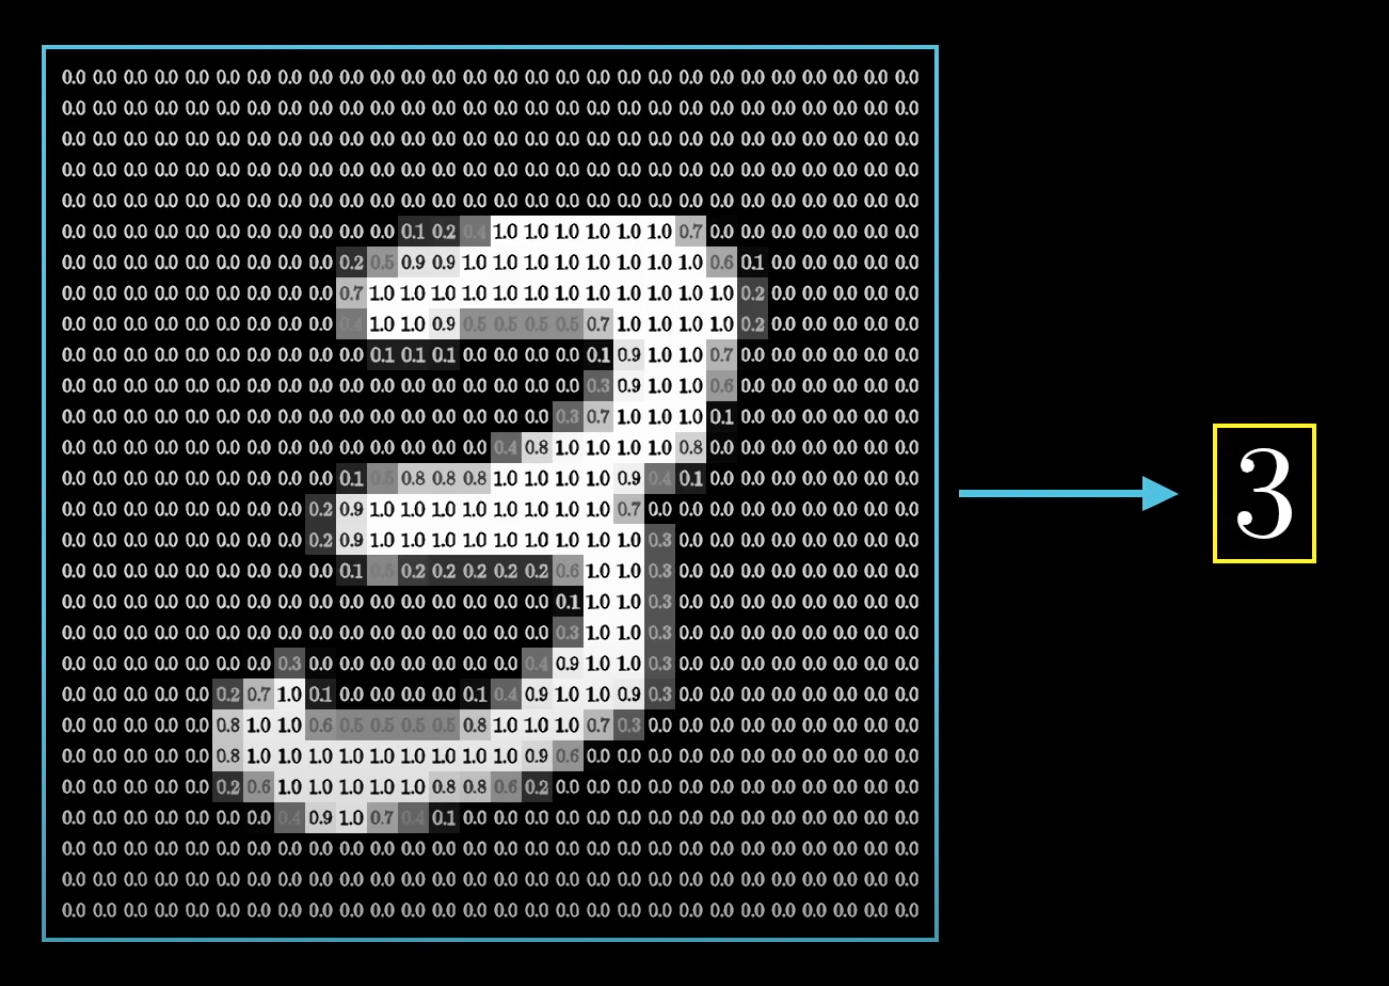
\includegraphics[width=6.8cm,keepaspectratio]{3.png}
\end{center}
\end{column}
\begin{column}{0.43\textwidth}
\small
Everyone in this room reads that instantly. Write down the rule you used.
\medskip

You cannot. And that is the point: the mapping from pixels to meaning is one you can \textbf{demonstrate} but not \textbf{state} --- exactly the position we are in with a policy function in twenty state variables.
\medskip

\begin{takeawaybox}\footnotesize
The next five frames are the whole intuition of this course's use of networks, in a setting where you already know the answer.
\end{takeawaybox}
\end{column}
\end{columns}
\end{frame}

%=============================================================================
\begin{frame}{The Same Thing, Written Down}
\begin{columns}[T]
\begin{column}{0.56\textwidth}
\small
\textbf{The data.} $\{(\mathbf{x}_i,y_i)\}_{i=1}^{N}$ with $\mathbf{x}_i\in[0,1]^{784}$ (a $28\times28$ image, flattened) and $y_i\in\{0,\dots,9\}$.
\medskip

\textbf{The map.}
\[
  f_\theta:\mathbf{x}\longmapsto\hat{\mathbf{p}}\in\Delta^{9},\qquad \hat y=\arg\max_k\hat p_k,
\]
where $\Delta^{9}$ is the probability simplex on ten classes.
\medskip

\textbf{The objective.}
\[
  \min_\theta\;\frac{1}{N}\sum_{i=1}^{N}\underbrace{\mathcal{L}\bigl(f_\theta(\mathbf{x}_i),y_i\bigr)}_{\text{cross-entropy}}+\lambda\lVert\theta\rVert_p
\]
\end{column}
\begin{column}{0.41\textwidth}
\begin{conceptbox}[title=\textbf{Look at the shape of it}]\small
An objective, a parameter vector, and a search. That is a structural estimation --- and $\theta$ has no interpretation whatsoever.
\end{conceptbox}
\medskip
\begin{examplebox}\footnotesize
\textbf{The search} is stochastic gradient descent and its variants (Adam, RMSProp) --- 7.A3, and exactly the \emph{first-order} method 4.A3 said it would have to be. And $\lambda\lVert\theta\rVert_p$ is all that stands between $784$ inputs and a perfect fit to noise.
\end{examplebox}
\end{column}
\end{columns}
\end{frame}

%=============================================================================
\begin{frame}{Why It Is Possible at All: Structure}
\begin{columns}[T]
\begin{column}{0.55\textwidth}
\small
A $28\times28$ image of independent random pixels is essentially never a digit. Handwriting is constrained:
\medskip
\begin{itemize}\small\setlength{\itemsep}{1.2mm}
  \item \textbf{anatomically} --- muscles, tendons and joints permit only certain strokes, so the patterns are systematic;
  \item \textbf{geometrically} --- a `0' has a closed loop, a `1' a vertical stroke, an `8' two stacked loops;
  \item \textbf{spatially} --- relative position, size and orientation preserve identity through a great deal of individual variation.
\end{itemize}
\end{column}
\begin{column}{0.42\textwidth}
\begin{takeawaybox}[title=\textbf{The economist's version}]\small
Economic theory constrains the space of plausible models in exactly this way. Structure is what makes a high-dimensional problem \textbf{effectively} low-dimensional.
\end{takeawaybox}
\medskip
\begin{conceptbox}\footnotesize
And the constraints can be \textbf{learned} rather than hand-built --- by data augmentation, by regularisation, and by the choice of architecture (7.A4).
\end{conceptbox}
\end{column}
\end{columns}
\end{frame}

%=============================================================================
\begin{frame}{From 784 Pixels to a Handful of Directions}
\begin{columns}[T]
\begin{column}{0.55\textwidth}
\small
\textbf{The manifold hypothesis.} Real digit images occupy a smooth $d$-dimensional manifold $\mathcal{M}\subset\mathbb{R}^{784}$ with $d\ll784$.
\medskip

In plain terms, only a few writing-style degrees of freedom matter: slant, stroke thickness, whether a loop closes, small translation. The other $780$-odd pixel directions are nearly empty.
\medskip

\textbf{The macro analogy is exact.} Finding a low-dimensional state inside a high-dimensional model is the same problem. A good representation keeps the few variables that matter for the next decision.
\end{column}
\begin{column}{0.42\textwidth}
\begin{conceptbox}[title=\textbf{You have done this before}]\small
Krusell--Smith replaces $\Gamma$ with its \textbf{mean} and finds that almost nothing is lost. That is a one-dimensional manifold hypothesis, asserted rather than learned.
\end{conceptbox}
\medskip
\begin{examplebox}\footnotesize
S8's DeepHAM does the learned version: \emph{generalised moments}, chosen by the network instead of by the modeller.
\end{examplebox}
\end{column}
\end{columns}
\end{frame}

%=============================================================================
\begin{frame}{The Encoder View}
\begin{columns}[T]
\begin{column}{0.57\textwidth}
\small
Split the map in two:
\[
  \mathbf{x}\;\xrightarrow{\;\pi:\mathbb{R}^{784}\to\mathbb{R}^{d}\;}\;\mathbf{z}\;\xrightarrow{\;g_\phi:\mathbb{R}^{d}\to\Delta^{9}\;}\;\hat{\mathbf{p}}
\]
\begin{itemize}\small\setlength{\itemsep}{1mm}
  \item $\pi$, the \textbf{encoder}, flattens the manifold into a latent code $\mathbf{z}$;
  \item $g_\phi$, the \textbf{head}, is one or two ordinary layers and a softmax.
\end{itemize}
\medskip

\textbf{Choices for $\pi$:} linear --- PCA, SVD, random projection; nonlinear --- an autoencoder, t-SNE, UMAP, or the early layers of a convolutional network.
\end{column}
\begin{column}{0.40\textwidth}
\begin{takeawaybox}[title=\textbf{The translation}]\small
The encoder learns a \textbf{nonlinear factor model} instead of imposing a fixed sufficient statistic.
\medskip
Sufficient statistics for prediction --- \emph{by learning}.
\end{takeawaybox}
\medskip
\begin{examplebox}\footnotesize
Rolf et al.\ (2021) found that for satellite imagery a \emph{random} $\pi$ plus a ridge regression is often enough (7.A4). The structure is doing the work, not the training.
\end{examplebox}
\end{column}
\end{columns}
\end{frame}

%=============================================================================
\begin{frame}{What the Input's Structure Decides}
\begin{center}
\resizebox{0.70\textwidth}{!}{%
\begin{tikzpicture}[
  every node/.style={font=\small},
  unit/.style={circle, draw, minimum size=0.52cm, inner sep=0pt, font=\scriptsize},
  inp/.style={unit, fill=blue!15},
  outp/.style={unit, fill=orange!20},
  init/.style={unit, fill=gray!15}
]
\begin{scope}
  \foreach \i in {1,...,4} \node[inp]  (a\i) at (\i*1.5, 0)   {$\mathbf{x}_{\i}$};
  \foreach \j in {1,...,4} \node[outp] (b\j) at (\j*1.5, 1.75) {$\mathbf{h}_{\j}$};
  \foreach \i in {1,...,4} \foreach \j in {1,...,4}
    \draw[gray!45, line width=0.25pt] (a\i) -- (b\j);
  \node[font=\footnotesize, align=center] at (3.75,-1.0)
    {(a) feedforward: $4\times4=16$ distinct weights\\change the sequence length and $\mathbf{W}$ changes shape};
\end{scope}
\begin{scope}[xshift=8.6cm]
  \foreach \i in {1,...,4} \node[inp]  (c\i) at (\i*1.5, 0)   {$\mathbf{x}_{\i}$};
  \foreach \j in {1,...,4} \node[outp] (d\j) at (\j*1.5, 1.75) {$\mathbf{h}_{\j}$};
  \node[init] (d0) at (0, 1.75) {$\mathbf{h}_{0}$};
  \foreach \i in {1,...,4}
    \draw[red!70!black, line width=0.7pt, -{Latex[length=1.8mm]}] (c\i) -- (d\i);
  \draw[blue!70!black, line width=0.7pt, -{Latex[length=1.8mm]}] (d0) -- (d1);
  \foreach \j in {1,2,3} {
    \pgfmathtruncatemacro{\k}{\j+1}
    \draw[blue!70!black, line width=0.7pt, -{Latex[length=1.8mm]}] (d\j) -- (d\k);
  }
  \node[font=\footnotesize, align=center] at (3.75,-1.0)
    {(b) recurrent: only $\mathbf{W}_x$ and $\mathbf{W}_h$\\the count does not depend on $T$};
  \begin{scope}[shift={(4.85,2.40)}]
    \draw[red!70!black,  line width=0.7pt, -{Latex[length=1.8mm]}] (0,0.30) -- (0.5,0.30);
      \node[right, font=\scriptsize] at (0.55,0.30) {$\mathbf{W}_x$};
    \draw[blue!70!black, line width=0.7pt, -{Latex[length=1.8mm]}] (0,0.02) -- (0.5,0.02);
      \node[right, font=\scriptsize] at (0.55,0.02) {$\mathbf{W}_h$};
  \end{scope}
\end{scope}
\end{tikzpicture}}
\end{center}
\vspace{-1mm}
\begin{columns}[T]
\begin{column}{0.49\textwidth}
\begin{conceptbox}\footnotesize
A digit is a \textbf{fixed-length} vector, so a feedforward layer is the natural reader: $784$ numbers in, one weight each.
\end{conceptbox}
\end{column}
\begin{column}{0.49\textwidth}
\begin{cautionbox}\footnotesize
\textbf{Text and a macro time series are not.} Order carries information, length varies, and a dense $\mathbf{W}$ sees neither. On the right, one $\mathbf{W}_x$ and one $\mathbf{W}_h$ serve \emph{any} $T$.
\end{cautionbox}
\end{column}
\end{columns}
\vspace{1mm}
\begin{takeawaybox}\footnotesize
\textbf{The representation comes first, and the architecture follows from it} --- which is why the encoder above was worth a frame. \textbf{7.A4} returns to this picture and makes the general statement: an architecture is a \emph{constraint} on $\mathbf{W}$.
\end{takeawaybox}
\end{frame}

%=============================================================================
\begin{frame}{A Network for Digits}
\begin{columns}[T]
\begin{column}{0.53\textwidth}
\small
\textbf{Architecture.}
\begin{itemize}\small\setlength{\itemsep}{1mm}
  \item input: $784$ units, one per pixel intensity;
  \item hidden: several layers, each applying a nonlinear transformation;
  \item output: $10$ units, one per class.
\end{itemize}
\medskip

\textbf{Nonlinearity} between the layers --- ReLU, sigmoid --- with depth and width chosen for the task. 7.A2 shows why the nonlinearity is not optional.
\end{column}
\begin{column}{0.44\textwidth}
\begin{conceptbox}[title=\textbf{The parallel that matters}]\small
The network's structure mirrors the recursive structure of a macro model: \textbf{state variables are transformed, layer by layer, into decisions} --- exactly as $k_t\mapsto(c_t,l_t)$ through a policy function.
\end{conceptbox}
\medskip
\begin{examplebox}\footnotesize
In 7.B1 the input layer is $(k,z)$ and the output layer is $c$. Nothing else about the object changes.
\end{examplebox}
\end{column}
\end{columns}
\end{frame}

%=============================================================================
\begin{frame}{The Sentence This Session Turns On}
\begin{columns}[T]
\begin{column}{0.55\textwidth}
\small
Session 5 wrote every approximation the same way:
\[
  d^{n}(x)=\sum_{i}\theta_i\,\psi_i(x),
\]
with $\{\psi_i\}$ --- monomials, Chebyshev polynomials, tent functions --- \textbf{fixed in advance}, and only $\theta$ unknown.
\medskip

A network is
\[
  \mathcal{N}(x;\theta),
\]
and the basis functions are \textbf{built out of $\theta$ as well}. Nothing else changes: it is still a family, still indexed by a parameter vector, still fitted by making something small.
\end{column}
\begin{column}{0.42\textwidth}
\begin{takeawaybox}[title=\textbf{The claim, precisely}]\small
The value of a neural network is \textbf{not} that it can approximate anything --- so can a polynomial.
\medskip
It is that the basis functions are \textbf{chosen by the optimisation} rather than by you.
\end{takeawaybox}
\medskip
\begin{cautionbox}\footnotesize
Which is also the bill: you lose the orthogonality, the conditioning guarantees and the error bounds that made 5.B3 comfortable. 7.A2 counts the cost.
\end{cautionbox}
\end{column}
\end{columns}
\vspace{1mm}
\src{The formulation follows Feng \& Miao, \emph{AI for Economists}, ch.~9 \S9.7; 5.B1 and 5.B2 promised this frame.}
\end{frame}

%=============================================================================
\begin{frame}{Takeaways, and What 7.A2 Opens}
\begin{columns}[T]
\begin{column}{0.55\textwidth}
\begin{takeawaybox}\small
\begin{itemize}\small\setlength{\itemsep}{1.2mm}
  \item ``Machine learning'' means three different jobs --- prediction, causation, \textbf{computation}. This course is doing the third, and there is no dataset in it.
  \item The curse of dimensionality bites twice: on the state space, and on the unfolding of uncertainty. A network answers both by \textbf{sampling instead of gridding}.
  \item The bottleneck moves from \emph{constructing a grid} to \emph{representing a function}.
  \item A network is the projection framework of 5.B1 with \textbf{one change}: the basis is learned.
\end{itemize}
\end{takeawaybox}
\end{column}
\begin{column}{0.42\textwidth}
\begin{conceptbox}[title=\textbf{Bridge to 7.A2}]\small
Open the box. What is a neuron, what does a layer do, and why is the nonlinearity between them the thing that makes depth mean anything?
\medskip
Then the two theorems: \textbf{universal approximation}, and \textbf{Barron's rate} --- one of which promises much less than it is usually said to.
\end{conceptbox}
\end{column}
\end{columns}
\end{frame}

\end{document}
